
\documentclass[./Thick_TQFTs_and_Quantum_Information.tex]{subfiles}

\begin{document}

\section{Paths for Parallel Transport}

In order to obtain linear maps by parallel transport on manifolds, we need
additional structure on top of connections. These are collections of paths on
manifolds along which we will parallel transport vectors in the fibres of a
bundle with connection. We shall now formalize this apparatus in terms of
categories. We will require a notion of graphs on manifolds whose vertices are
points, possibly repeated, on the manifold and whose edges are paths on the
manifold.

\subsection{Graphs Encoding Algebraic Expressions}

We will now describe a method of encoding expressions involving tensor products,
point-wise algebra products and composition of linear maps $A \to A$ for some
algebra $A$, using directed graphs. As a matter of convention, we will take all
graphs to mean directed acyclic graphs where we do not allow parallel edges or
self-loops. However, we do allow the underlying undirected graph of any directed
graph to be a forest. Given a graph $G = (V, E)$, we will write $V = V(G)$ and
$E = E(G)$.

\begin{exm}\label{exm:egraph1}
Consider a graph consisting of nine vertices $1, \dots, 9$ with
$V_1 = \set{1, 2}$, $V_2 = \set{3, 4}$, $V_4 = \set{5, 6, 7}$ and
$V_4 = \set{8, 9}$, along with edges:
\[\begin{array}{ccccc}
  (1, 3) &,& (1, 4) &,& (2, 3),\\
  (3, 5) &,& (3, 6) &,& (4, 7),\\
  (5, 8) &,& (6, 9) &,& (7, 9)
\end{array}\]
We visualize this graph as follows:
\[\begin{tikzpicture}[baseline=(a).base]
\node[scale=\diagscale] (a) at (0, 0){
\begin{tikzcd}[column sep=huge, row sep=tiny]
                  &                   & 5 \ar[rd] &   \\
1 \ar[r] \ar[rdd] & 3 \ar[ru] \ar[rd] &           & 8 \\
                  &                   & 6 \ar[rd] &   \\
2 \ar[ruu]        & 4 \ar[rd]         &           & 9 \\
                  &                   & 7 \ar[ur] &
\end{tikzcd}
};
\end{tikzpicture}\]
In particular, this diagram gives a topological ordering of vertices. We then
observe that we can use this graph to generate an algebraic expression of the
form:
\[
  ((5, 8) \tensor ((6, 9) \cdot (7, 9))) \circ
  ((3, 5) \tensor (3, 6) \tensor (4, 7)) \circ
  (((1, 3) \cdot (2, 3)) \tensor (1, 4))
\]
where the rule is roughly as follows: we infix $(6, 9)$ and $(7, 9)$ with
`$\cdot$' because they share the same target vertex and we call $9$ the target
vertex of $(6, 9) \cdot (7, 9)$; we infix the expressions $(6, 9) \cdot (7, 9)$
and $(5, 8)$ with a `$\tensor$' because they do not share the same target vertex
and we call the expression $5 \tensor 6 \tensor 7$ the source and the expression
$8 \tensor 9$ the target of the expression
$(5, 8) \tensor ((6, 9) \cdot (7, 9))$. For expressions $E_1$ and $E_2$ such
that the target of $E_1$ is the source of $E_2$, we call these expressions
composeable and we form the new expression $E_2 \circ E_1$. This yields the
whole expression above.

One sees readily that the edges can be replaced with paths in a manifold $M$
equipped with an $A$--fibred bundle with connection. These paths can then be
replaced replaced with linear maps $A \to A$ yielding a linear map corresponding
to the expression. We can associate this linear map to $M$ in some notion of
TQFT. This will later motivate us to define an algorithm for obtaining a
canonical expression from an expression graph.
\end{exm}

This motivates the following definitions, some of which are standard but we
include for convenience.

\begin{defn}[Level Ordering]
Given a directed acyclic graph $G = (V, E)$, we let $V_1$ denote the subset of
$V$ consisting of vertices with no incoming edges. We let $V_{k + 1}$ denote the
subset of $V$ consisting of vertices that have incoming edges only from vertices
in $V_{1} \cup V_{2} \cup \cdots \cup V_{k}$. We note that the $V_i$'s are
disjoint for distinct $i$ such that there exist finitely many $V_i$
such that $V = \coprod_{i = 1}^{N} V_i$ for some $N \in \N$. Then, the $V_i$'s
are called the levels of $G$ and the set $\mathcal{V} = \set{V_1, \dots, V_N}$,
a level ordering of $G$. In this case, we call $G$ level-ordered.

Given a level ordering as this, we can define a level
function $l_{\mathcal{V}} : V \to \set{1, \dots, k}$, given by
$l_{\mathcal{V}}(v) = i$ if and only if $v \in V_i$.
\end{defn}

\begin{rmk}
The existence of a level ordering of a directed acyclic graph is well-known --
consider any topological sorting algorithm -- but these orderings need not be
unique -- consider the disjoint union of two directed acyclic graphs.
\end{rmk}

\begin{rmk}\label{rmk:lgraph_edge}
We also note that if a vertex has no incoming nor outgoing edges, then it is
placed at the lowest level. Vertices at any level cannot have outgoing edges to
a lower level, for if they do, then the graph has a cycle. Finally, we note that
if a vertex at some level has no edge from the immediate preceding level, we can
move it to that level. Hence, we may assume that each vertex not at the first
level has at least one edge from the immediate preceding level.
\end{rmk}

\begin{exm}
A level-ordering of the graph in example \ref{exm:egraph1} is:
\[
  V_1 = \set{1, 2}, V_2 = \set{3, 4}, V_3 = \set{5, 6, 7}, V_4 = \set{8, 9}
\]
\end{exm}

\begin{defn}[Expression of a Graph]
Given a graph $G$ with a chosen level ordering $\set[V_i]{i = 1, \dots, N}$
along with a chosen total ordering
$V_i = \set{v_{i, 1}, v_{i, 2}, \dots, v_{i, k_i}}$ of each level, we define:
\begin{enumerate}[(i)]
\setlength{\itemsep}{0pt}
\item For $j \in \set{1, \dots, k_1}$, the expression associated to $v_{1, j}$
is:
\[
  \Exp{G}_{1, j} := v_{1, j}\footnote{We take this vertex as a formal symbol.}
\]
The expression associated to the layer $V_1$ is:
\[
  \Exp{G}_1 := v_{1, 1} \tensor \cdots \tensor v_{1, k_1}
\]

\item For
$i \in \set{2, \dots, N}$,
$j \in \set{1, \dots, k_i}$,
let $\set{e_1, e_2, \dots, e_q}$ be the set of incoming edges on $v_{i, j}$,
ordered by the source vertices. Then, the expression associated to $v_{i, j}$
is:
\[
  \Exp{G}_{i, j} := e_1 \cdot e_2 \cdot \cdots \cdot e_q
\]
The expression associated to the layer $V_{i}$ is:
\[
  \Exp{G}_{i} := \Exp{G}_{i, 1} \tensor \Exp{G}_{i, 2} \tensor \cdots
                 \tensor \Exp{G}_{i, k_{i}}
\]

\item If $N = 0$, the expression associated to $G$ is:
\[
  \Exp{G} := \varnothing
\]
If $N = 1$, the expression associated to $G$ is:
\[
  \Exp{G} := \Exp{G}_1
\]
If $N > 1$, the expression associated to $G$ is:
\[
  \Exp{G} := \Exp{G}_N \circ \Exp{G}_{N - 1} \circ \cdots \circ \Exp{G}_{2}
\]
\end{enumerate}
Then, $\Exp{G}$ is called the expression of $G$ for the given level ordering and
the given total orderings of the levels.
\end{defn}

From this definition it is clear that level-ordered sets encode algebraic
expressions of the form we saw in example \ref{exm:egraph1}.

\subsection{Disjoint Unions and Gluings}

For defining a disjoint union of level-ordered graphs, we require an operation
of level orders that yields a level ordering of the disjoint union of the
graphs. We see an example first.

\begin{exm}\label{exm:lgraph_disjunion}
Consider the graph in example \ref{exm:egraph1} -- call it $G$ -- along with the
following graph $H$:
\[\begin{tikzpicture}[baseline=(a).base]
\node[scale=\diagscale] (a) at (0, 0){
\begin{tikzcd}[column sep=huge, row sep=tiny]
                                &                    & 5' \\
1' \ar[rru, bend left] \ar[rdd] & 3' \ar[ru] \ar[rd] &    \\
                                &                    & 6' \\
2' \ar[ruu]                     & 4' \ar[rd] \ar[ru] &    \\
                                &                    & 7'
\end{tikzcd}
};
\end{tikzpicture}\]
We then observe the following diagram of $G \amalg H$:
\[\begin{tikzpicture}[baseline=(a).base]
\node[scale=\diagscale] (a) at (0, 0){
\begin{tikzcd}[column sep=huge, row sep=tiny]
                                    &                      & 5 \ar[rd] &    \\
1 \ar[r] \ar[rdd]                   & 3 \ar[ru] \ar[rd]    &           & 8  \\
                                    &                      & 6 \ar[rd] &    \\
2 \ar[ruu]                          & 4 \ar[rd]            &           & 9  \\
                                    &                      & 7 \ar[ur] &    \\
                                    &                      &           &    \\
                                    &                      &           & 5' \\
1' \ar[rrru, bend left=20] \ar[rdd] & 3' \ar[rru] \ar[rrd] &           &    \\
                                    &                      &           & 6' \\
2' \ar[ruu]                         & 4' \ar[rrd] \ar[rru] &           &    \\
                                    &                      &           & 7'
\end{tikzcd}
};
\end{tikzpicture}\]
This suggests one possible operation on level sets which yields a level
ordering. We define this next.
\end{exm}

\begin{cor}
Let $(G, \mathcal{V} = \set{V_i}_{i = 1}^{N})$ and
$(H, \mathcal{W} = \set{W_i}_{i = 1}^{M})$ be level-ordered
graphs. If $M \leq N$, the following set is a level ordering of $G \amalg H$:
\[
  \mathcal{V} \tensor \mathcal{W} :=
  \set{V_1 \amalg W_1, V_2 \amalg W_2, \dots, V_{M - 1} \amalg W_{M - 1},
  V_M, \dots, V_{N - 1}, V_N \amalg W_M}
\]
If $N \leq M$, the following set is a level ordering of $G \amalg H$:
\[
  \mathcal{V} \tensor \mathcal{W} :=
  \set{V_1 \amalg W_1, V_2 \amalg W_2, \dots, V_{N - 1} \amalg W_{N - 1},
  W_N, \dots, W_{M - 1}, V_N \amalg W_M}
\]
If $N = M$, these two descriptions coincide.
\end{cor}

This allows us to define a disjoint union of level-ordered graphs.
\begin{defn}
For level-ordered graphs $(G, \mathcal{V})$ and $(H, \mathcal{W})$, we define
\[
  (G, \mathcal{V}) \tensor (H, \mathcal{W}) :=
    (G \amalg H, \mathcal{V} \tensor \mathcal{W})
\]
to be the disjoint union.
\end{defn}

\begin{rmk}
We notice that if we choose total orderings of levels, then this disjoint union
again gives total orderings of levels.
\end{rmk}

To see the associativity and unitality of this operation up to ``coherent
isomorphism'', we require a notion of morphism of level-ordered graphs. We
define this now.

\begin{defn}[Level Homomorphism]
Let $(G, \mathcal{V} = \set{V_i}_{i = 1}^{N})$ and
$(H, \mathcal{W} = \set{W_i}_{i = 1}^{M})$ be level-ordered
graphs. Then, a graph homomorphism $h : G \to H$ satisfying:
\[
  l_{\mathcal{V}}(u) = l_{\mathcal{V}}(v)
  \implies l_{\mathcal{W}}(h(u)) = l_{\mathcal{W}}(h(v))
\]
\end{defn}

It is then straightforward to verify that the associator and unitor isomorphisms
for the disjoint union of vertex sets are level homomorphisms of graphs -- this
is an exercise similar to verifying that disjoint unions of connections are
associative and unital, as we saw in \S\ref{subsec:connctg}. We then proceed to
define a gluing of level-ordered graphs.

\begin{defn}[Source and Target]
Let $(G, \mathcal{V} = \set{V_i}_{i = 1}^{N})$ be a level-ordered graph. Then,
we define $V_1$ to be the source graph $S(G)$ of $G$ and $V_N$ to be the target
graph $T(G)$ of $G$.
\end{defn}

It is obvious that $S(G)$ and $T(G)$ are single-level level-ordered graphs with
obvious inclusion homomorphisms that are also level homomorphisms. However,
gluing at source target-ends is not well-defined, unless we have a unique
isomorphism between the source of one graph to the target of another. This is
another reason we should consider total orderings of the levels. Recall that we
required total orderings of levels to define expressions of level-ordered
graphs. Hence, we define the following subclass of level-ordered graphs.

\begin{defn}[Expression Graph]
A level-ordered graph $(G, \mathcal{V})$ equipped with a total ordering of its
levels is called an expression graphs.
\end{defn}

\begin{defn}[Expression Homomorphism]
A level homomorphism that is order-preserving on levels is called an expression
homomorphism.
\end{defn}

We then observe that $S(G)$ and $T(G)$ are totally ordered for any expression
graph $G$. Then we have the following theorem.

\begin{thm}\label{thm:expiso_unique}
Expression isomorphisms are unique.
\end{thm}
\begin{proof}
Let $f : (G, \mathcal{V}) \to (H, \mathcal{W})$ be an expression isomorphism,
where $\mathcal{V} = \set{V_i}_{i = 1}^{N}$ and
$\mathcal{W} = \set{W_j}_{i = 1}^{M}$. By remark \ref{rmk:lgraph_edge}, we have
a path $v_1, v_2, \dots, v_N$ in $G$ with $v_i \in V_i$. Then,
$f(v_1), f(v_2), \dots, f(v_N)$ is a path in $H$ with $f(v_i) \in W_{j(i)}$
for some strictly increasing finite sequence
$j : \set{1, \dots, N} \to \set{1, \dots, M}$, since edges always go forward in
levels. This shows that $N \leq M$. Using $f^{-1}$ and a path in $H$, we can
show that $M \leq N$ so that $N = M$. This also shows that $f(v_1) \in W_1$ and
hence $f(v_i) \in W_i$ for each $i$, by counting.

Now, if there is another vertex $v'_i \in V_i$ for any $i$, we have
$l_{\mathcal{V}}(v'_i) = l_{\mathcal{V}}(v_i) \implies
l_{\mathcal{V}}(f(v'_i)) = l_{\mathcal{V}}(f(v_i))$. Thus, $f(V_i) \subset W_i$.
Using the same argument with $f^{-1}$, we have $f^{-1}(W_i) \subset V_i$. Hence,
we must have $f(V_i) = W_i$ for all $i$. For any other isomorphism $f'$ with the
same domain and codomain, we can similarly show that $f'(V_i) = W_i$ for all
$i$. Finally, since order-preserving bijections between finite, totally ordered
sets -- the levels -- are unique, we must have $f = f'$ on all $V_i$. Thus,
$f = f'$ on all of $G$.
\end{proof}

\begin{defn}[Gluing of Expression Graphs]
Let $(G, \mathcal{V} = \set{V_i}_{i = 1}^{N})$ and
$(H, \mathcal{W} = \set{W_i}_{i = 1}^{M})$ be level-ordered
graphs such that there is a unique expression isomorphism
\[
  \psi_{G, H} : W_1 = S(H) \to T(G) = V_N
\]
Then, we say that $G$ and $H$ are gluable at $S(H) \cong T(G)$. We define the
pushout of the following span in $\Set$ to be the gluing $H * G$ of graphs.
\[
  H \hot S(H) \to[\phi] T(G) \hto G
\]
$H * G$ has the obvious level-ordering:
\[
  \mathcal{W} * \mathcal{V} :=
  \set{V_1, \dots, V_N \cong W_1, W_2, \dots, W_M}
\]
We call $(H * G, \mathcal{W} * \mathcal{V})$ the gluing or composite of the
given level-ordered graphs.
\end{defn}

\begin{exm}
Consider $G$ and $H$ as in example \ref{exm:lgraph_disjunion}. We have the
following diagram of $H * G$:
\[\begin{tikzpicture}[baseline=(a).base]
\node[scale=\diagscale] (a) at (0, 0){
\begin{tikzcd}[column sep=huge, row sep=tiny]
                  &                   & 5 \ar[rd] &                                     &                    & 5' \\
1 \ar[r] \ar[rdd] & 3 \ar[ru] \ar[rd] &           & 8 \cong 1' \ar[rru, bend left] \ar[rdd] & 3' \ar[ru] \ar[rd] &    \\
                  &                   & 6 \ar[rd] &                                     &                    & 6' \\
2 \ar[ruu]        & 4 \ar[rd]         &           & 9 \cong 2' \ar[ruu]                     & 4' \ar[rd] \ar[ru] &    \\
                  &                   & 7 \ar[ur] &                                     &                    & 7'
\end{tikzcd}
};
\end{tikzpicture}\]
\end{exm}

It is then easy to verify that this gluing is associative and unital up to
coherent isomorphism much like the disjoint union. In fact, associators and
unitors of the disjoint union of level-ordered graphs also expression
isomorphisms. We can further verify that the data of expression graphs defined
so far form a monoidal double category whose objects are finite, ordered sets,
vertical $1$--morphisms are unique order isomorphisms, horizontal $1$--morphisms
$G : U \to V$ are expression graphs $G$ with $S(G) \cong U$ and $T(G) \cong V$,
and $2$--morphisms are expression isomorphisms, with horizontal composition
given by gluing and monoidal product given by disjoint union as defined above.

\TODO{Maybe, we should have an appendix entry for the proof.}

\subsection{Some Constructs on Expressions}

We define some basic constructs on expressions obtained from expression graphs.

\begin{defn}[Equality of Expressions]
If $E_1$ and $E_2$ are expressions such that there exist isomorphic
expression graphs $G$ and $H$ with $\Exp{G} = E_1$ and
$\Exp{H} = E_2$, then we say that $E_1$ and $E_2$ are equal.
\end{defn}

\begin{defn}[Expression Composition]
Let $G$ and $H$ be expression graphs gluable at $S(H) \cong T(G)$. Then, we
define:
\[
  \Exp{H} \circ \Exp{G} := \Exp{H * G}
\]
\end{defn}

\begin{defn}[Expression Tensor Product]
Let $G$ and $H$ be expression graphs. We define:
\[
  \Exp{G} \tensor \Exp{H} := \Exp{G \tensor H}
\]
\end{defn}

\begin{defn}[Expression Substitution]
Given an expression graph $G$, we write
\[
  \Exp{G}[f] \text{ or } \Exp{G}[f(u, v)] \text{ or } \Exp{G}[(u, v)/f(u, v)]
\]
to denote the expression obtained by replacing each edge $(u, v) \in G$ in
$\Exp{G}$ with some string of symbols $f(u, v)$, depending on $(u, v)$.
\end{defn}

\subsection{Geometric Realization}

We wish to use expression graphs to generate linear maps by viewing the edges as
paths in a manifold equipped with an algebra-fibred bundle with connection,
taking their associated parallel transport maps, and combining these maps in a
pattern encoded in the expression graph. To accomplish this, we use the
following simple notion of geometric realization of graphs.

\begin{defn}[Geometric Graph]
A graph in a manifold $M$ or a geometric graph is a graph $G = (V, E)$ equipped
with a function $\gamma : E \to C^0(I, M)$, called a geometric realization of
$G$. We call $M$ the realizing manifold of $G$ under $\gamma$. For an edge from
$u$ to $v$ we write $\gamma_{u, v}$ to denote the path associated to that edge.
\end{defn}

\begin{rmk}
A geometric graph is essentially a collection of paths in a manifold but we
consider one or more copies of each path and ``identify'' their end-points in a
pattern encoded by a graph, even though these paths need not share end-points --
that is, we do not strictly require $\gamma_{u, v}(1) = \gamma_{v, w}(0)$. We
will see that this relaxation is essential to defining our notion of TQFTs. We
will ultimately be interested in expression graphs in manifolds, which will
provide us with a way to associate linear maps to manifolds.
\end{rmk}

\begin{exm}\label{exm:geomegraph}
Consider the graph in example \ref{exm:egraph1}. Then, we consider a mapping of
the edges to paths on a surface as shown below.\footnote{This diagram was
generated using \cite{Mathcha}.} Note that here we have
$\gamma_{u, v}(1) = \gamma_{v, w}(0)$ for most points but not all -- for
instance, $\gamma_{2, 3}$ and $\gamma_{3, 5}$ do not share any end-points.
\begin{figure}[H]
\begin{center}

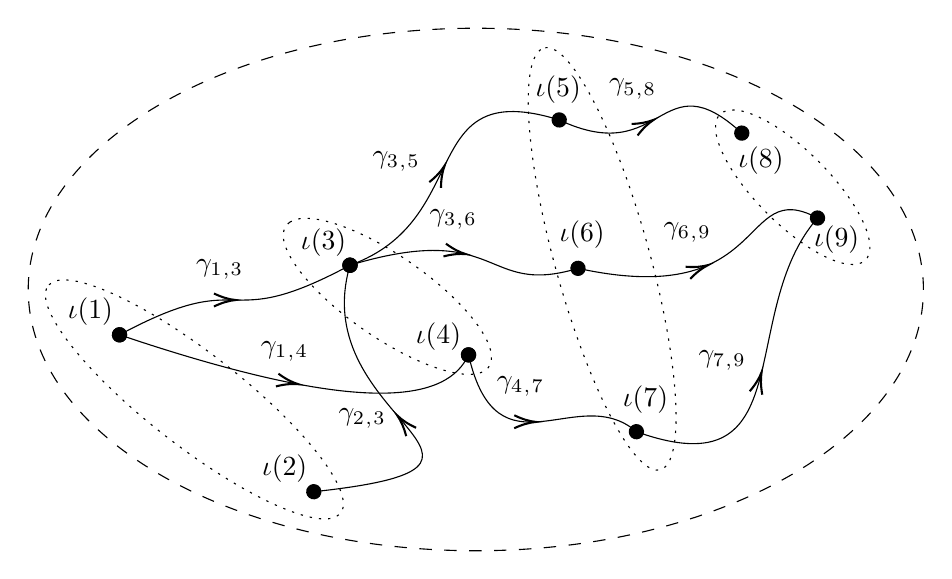
\begin{tikzpicture}[x=0.75pt,y=0.75pt,yscale=-0.95,xscale=0.95]
%uncomment if require: \path (0,281); %set diagram left start at 0, and has height of 281

%Shape: Ellipse [id:dp45216116111361904] 
\draw  [dash pattern={on 4.5pt off 4.5pt}] (6,138.5) .. controls (6,65.32) and (107.63,6) .. (233,6) .. controls (358.37,6) and (460,65.32) .. (460,138.5) .. controls (460,211.68) and (358.37,271) .. (233,271) .. controls (107.63,271) and (6,211.68) .. (6,138.5) -- cycle ;
%Curve Lines [id:da12378300176275903] 
\draw    (52.31,161.49) .. controls (119.1,125.59) and (102.4,162.09) .. (169.19,126.19) ;
\draw [shift={(169.19,126.19)}, rotate = 331.74] [color={rgb, 255:red, 0; green, 0; blue, 0 }  ][fill={rgb, 255:red, 0; green, 0; blue, 0 }  ][line width=0.75]      (0, 0) circle [x radius= 3.35, y radius= 3.35]   ;
\draw [shift={(111.13,143.84)}, rotate = 180.1] [color={rgb, 255:red, 0; green, 0; blue, 0 }  ][line width=0.75]    (10.93,-3.29) .. controls (6.95,-1.4) and (3.31,-0.3) .. (0,0) .. controls (3.31,0.3) and (6.95,1.4) .. (10.93,3.29)   ;
\draw [shift={(52.31,161.49)}, rotate = 331.74] [color={rgb, 255:red, 0; green, 0; blue, 0 }  ][fill={rgb, 255:red, 0; green, 0; blue, 0 }  ][line width=0.75]      (0, 0) circle [x radius= 3.35, y radius= 3.35]   ;
%Curve Lines [id:da3902364739215902] 
\draw    (169.19,126.19) .. controls (233.04,103.33) and (202.45,29.92) .. (275.29,52.51) ;
\draw [shift={(275.29,52.51)}, rotate = 17.23] [color={rgb, 255:red, 0; green, 0; blue, 0 }  ][fill={rgb, 255:red, 0; green, 0; blue, 0 }  ][line width=0.75]      (0, 0) circle [x radius= 3.35, y radius= 3.35]   ;
\draw [shift={(217.18,75.67)}, rotate = 476.11] [color={rgb, 255:red, 0; green, 0; blue, 0 }  ][line width=0.75]    (10.93,-3.29) .. controls (6.95,-1.4) and (3.31,-0.3) .. (0,0) .. controls (3.31,0.3) and (6.95,1.4) .. (10.93,3.29)   ;
\draw [shift={(169.19,126.19)}, rotate = 340.3] [color={rgb, 255:red, 0; green, 0; blue, 0 }  ][fill={rgb, 255:red, 0; green, 0; blue, 0 }  ][line width=0.75]      (0, 0) circle [x radius= 3.35, y radius= 3.35]   ;
%Curve Lines [id:da5125133831866234] 
\draw    (52.31,161.49) .. controls (178.45,204.05) and (218.84,194.46) .. (229.3,171.66) ;
\draw [shift={(229.3,171.66)}, rotate = 294.65] [color={rgb, 255:red, 0; green, 0; blue, 0 }  ][fill={rgb, 255:red, 0; green, 0; blue, 0 }  ][line width=0.75]      (0, 0) circle [x radius= 3.35, y radius= 3.35]   ;
\draw [shift={(142.99,186.54)}, rotate = 191.16] [color={rgb, 255:red, 0; green, 0; blue, 0 }  ][line width=0.75]    (10.93,-3.29) .. controls (6.95,-1.4) and (3.31,-0.3) .. (0,0) .. controls (3.31,0.3) and (6.95,1.4) .. (10.93,3.29)   ;
\draw [shift={(52.31,161.49)}, rotate = 18.65] [color={rgb, 255:red, 0; green, 0; blue, 0 }  ][fill={rgb, 255:red, 0; green, 0; blue, 0 }  ][line width=0.75]      (0, 0) circle [x radius= 3.35, y radius= 3.35]   ;
%Curve Lines [id:da9936282267570157] 
\draw    (150.83,241.06) .. controls (275.76,227.54) and (145.96,205.62) .. (169.19,126.19) ;
\draw [shift={(169.19,126.19)}, rotate = 286.3] [color={rgb, 255:red, 0; green, 0; blue, 0 }  ][fill={rgb, 255:red, 0; green, 0; blue, 0 }  ][line width=0.75]      (0, 0) circle [x radius= 3.35, y radius= 3.35]   ;
\draw [shift={(193.16,202.39)}, rotate = 409.89] [color={rgb, 255:red, 0; green, 0; blue, 0 }  ][line width=0.75]    (10.93,-3.29) .. controls (6.95,-1.4) and (3.31,-0.3) .. (0,0) .. controls (3.31,0.3) and (6.95,1.4) .. (10.93,3.29)   ;
\draw [shift={(150.83,241.06)}, rotate = 353.83] [color={rgb, 255:red, 0; green, 0; blue, 0 }  ][fill={rgb, 255:red, 0; green, 0; blue, 0 }  ][line width=0.75]      (0, 0) circle [x radius= 3.35, y radius= 3.35]   ;
%Curve Lines [id:da37329721640419344] 
\draw    (229.3,171.66) .. controls (243.97,235.64) and (284.76,184.82) .. (314.44,210.62) ;
\draw [shift={(314.44,210.62)}, rotate = 41] [color={rgb, 255:red, 0; green, 0; blue, 0 }  ][fill={rgb, 255:red, 0; green, 0; blue, 0 }  ][line width=0.75]      (0, 0) circle [x radius= 3.35, y radius= 3.35]   ;
\draw [shift={(263.43,205.67)}, rotate = 180.44] [color={rgb, 255:red, 0; green, 0; blue, 0 }  ][line width=0.75]    (10.93,-3.29) .. controls (6.95,-1.4) and (3.31,-0.3) .. (0,0) .. controls (3.31,0.3) and (6.95,1.4) .. (10.93,3.29)   ;
\draw [shift={(229.3,171.66)}, rotate = 77.09] [color={rgb, 255:red, 0; green, 0; blue, 0 }  ][fill={rgb, 255:red, 0; green, 0; blue, 0 }  ][line width=0.75]      (0, 0) circle [x radius= 3.35, y radius= 3.35]   ;
%Curve Lines [id:da6402293447536181] 
\draw    (169.19,126.19) .. controls (246.58,102.99) and (236.29,142.42) .. (284.82,127.77) ;
\draw [shift={(284.82,127.77)}, rotate = 343.19] [color={rgb, 255:red, 0; green, 0; blue, 0 }  ][fill={rgb, 255:red, 0; green, 0; blue, 0 }  ][line width=0.75]      (0, 0) circle [x radius= 3.35, y radius= 3.35]   ;
\draw [shift={(227.95,120.58)}, rotate = 190.98] [color={rgb, 255:red, 0; green, 0; blue, 0 }  ][line width=0.75]    (10.93,-3.29) .. controls (6.95,-1.4) and (3.31,-0.3) .. (0,0) .. controls (3.31,0.3) and (6.95,1.4) .. (10.93,3.29)   ;
%Curve Lines [id:da7275544623824886] 
\draw    (314.44,210.62) .. controls (399.23,240.98) and (364.55,150.12) .. (406.29,102.26) ;
\draw [shift={(406.29,102.26)}, rotate = 311.09] [color={rgb, 255:red, 0; green, 0; blue, 0 }  ][fill={rgb, 255:red, 0; green, 0; blue, 0 }  ][line width=0.75]      (0, 0) circle [x radius= 3.35, y radius= 3.35]   ;
\draw [shift={(377.94,180.41)}, rotate = 465.08] [color={rgb, 255:red, 0; green, 0; blue, 0 }  ][line width=0.75]    (10.93,-3.29) .. controls (6.95,-1.4) and (3.31,-0.3) .. (0,0) .. controls (3.31,0.3) and (6.95,1.4) .. (10.93,3.29)   ;
%Shape: Ellipse [id:dp21247917365246105] 
\draw  [color={rgb, 255:red, 0; green, 0; blue, 0 }  ,draw opacity=1 ][dash pattern={on 0.84pt off 2.51pt}] (16.54,136.11) .. controls (25.63,126.66) and (66.01,145.03) .. (106.72,177.14) .. controls (147.44,209.25) and (173.08,242.94) .. (163.99,252.39) .. controls (154.9,261.85) and (114.52,243.48) .. (73.81,211.37) .. controls (33.09,179.26) and (7.45,145.57) .. (16.54,136.11) -- cycle ;
%Curve Lines [id:da7880732583039812] 
\draw    (275.29,52.51) .. controls (328.72,77.63) and (326.15,20.9) .. (367.89,59.19) ;
\draw [shift={(367.89,59.19)}, rotate = 42.53] [color={rgb, 255:red, 0; green, 0; blue, 0 }  ][fill={rgb, 255:red, 0; green, 0; blue, 0 }  ][line width=0.75]      (0, 0) circle [x radius= 3.35, y radius= 3.35]   ;
\draw [shift={(323.24,52.43)}, rotate = 512.6] [color={rgb, 255:red, 0; green, 0; blue, 0 }  ][line width=0.75]    (10.93,-3.29) .. controls (6.95,-1.4) and (3.31,-0.3) .. (0,0) .. controls (3.31,0.3) and (6.95,1.4) .. (10.93,3.29)   ;
%Curve Lines [id:da726151739669847] 
\draw    (284.82,127.77) .. controls (383.33,149.3) and (366.22,80.72) .. (406.29,102.26) ;
\draw [shift={(350.78,126.12)}, rotate = 518.99] [color={rgb, 255:red, 0; green, 0; blue, 0 }  ][line width=0.75]    (10.93,-3.29) .. controls (6.95,-1.4) and (3.31,-0.3) .. (0,0) .. controls (3.31,0.3) and (6.95,1.4) .. (10.93,3.29)   ;
%Shape: Ellipse [id:dp20693904539608654] 
\draw  [color={rgb, 255:red, 0; green, 0; blue, 0 }  ,draw opacity=1 ][dash pattern={on 0.84pt off 2.51pt}] (138.62,104.37) .. controls (148.74,97.58) and (179.13,108.92) .. (206.48,129.69) .. controls (233.84,150.47) and (247.81,172.81) .. (237.69,179.59) .. controls (227.57,186.38) and (197.19,175.04) .. (169.83,154.27) .. controls (142.47,133.49) and (128.5,111.15) .. (138.62,104.37) -- cycle ;
%Shape: Ellipse [id:dp4442811176180146] 
\draw  [dash pattern={on 0.84pt off 2.51pt}] (268.26,15.88) .. controls (281.5,13.99) and (305.14,60.41) .. (321.05,119.55) .. controls (336.96,178.69) and (339.13,228.17) .. (325.89,230.05) .. controls (312.64,231.94) and (289.01,185.52) .. (273.09,126.38) .. controls (257.18,67.24) and (255.02,17.76) .. (268.26,15.88) -- cycle ;
%Shape: Ellipse [id:dp2537302094398456] 
\draw  [dash pattern={on 0.84pt off 2.51pt}] (358.5,48.46) .. controls (367.96,43.55) and (391.4,56.66) .. (410.84,77.74) .. controls (430.28,98.83) and (438.37,119.9) .. (428.91,124.82) .. controls (419.45,129.73) and (396.01,116.62) .. (376.57,95.54) .. controls (357.13,74.45) and (349.04,53.37) .. (358.5,48.46) -- cycle ;

% Text Node
\draw (50.31,158.09) node [anchor=south east] [inner sep=0.75pt]    {$\iota ( 1)$};
% Text Node
\draw (148.83,237.66) node [anchor=south east] [inner sep=0.75pt]    {$\iota ( 2)$};
% Text Node
\draw (168.57,122.92) node [anchor=south east] [inner sep=0.75pt]    {$\iota ( 3)$};
% Text Node
\draw (226.84,170.66) node [anchor=south east] [inner sep=0.75pt]    {$\iota ( 4)$};
% Text Node
\draw (262.03,45.25) node [anchor=south west] [inner sep=0.75pt]    {$\iota ( 5)$};
% Text Node
\draw (274.13,119.08) node [anchor=south west] [inner sep=0.75pt]    {$\iota ( 6)$};
% Text Node
\draw (306.28,202.6) node [anchor=south west] [inner sep=0.75pt]    {$\iota ( 7)$};
% Text Node
\draw (364.82,65) node [anchor=north west][inner sep=0.75pt]    {$\iota ( 8)$};
% Text Node
\draw (403.23,105) node [anchor=north west][inner sep=0.75pt]    {$\iota ( 9)$};
% Text Node
\draw (89.78,121.75) node [anchor=north west][inner sep=0.75pt]    {$\gamma _{1}{}_{,}{}_{3}$};
% Text Node
\draw (122.67,163.43) node [anchor=north west][inner sep=0.75pt]    {$\gamma _{1}{}_{,}{}_{4}$};
% Text Node
\draw (162.08,197.67) node [anchor=north west][inner sep=0.75pt]    {$\gamma _{2}{}_{,}{}_{3}$};
% Text Node
\draw (179.33,67.29) node [anchor=north west][inner sep=0.75pt]    {$\gamma _{3}{}_{,}{}_{5}$};
% Text Node
\draw (208.3,96.52) node [anchor=north west][inner sep=0.75pt]    {$\gamma _{3}{}_{,}{}_{6}$};
% Text Node
\draw (242.33,181.1) node [anchor=north west][inner sep=0.75pt]    {$\gamma _{4}{}_{,}{}_{7}$};
% Text Node
\draw (299.22,30.41) node [anchor=north west][inner sep=0.75pt]    {$\gamma _{5}{}_{,}{}_{8}$};
% Text Node
\draw (326.9,103.09) node [anchor=north west][inner sep=0.75pt]    {$\gamma _{6}{}_{,}{}_{9}$};
% Text Node
\draw (344.63,168.21) node [anchor=north west][inner sep=0.75pt]    {$\gamma _{7}{}_{,}{}_{9}$};


\end{tikzpicture}


\end{center}
\caption{An elementary transport graph}
\end{figure}
We notice that the same algebraic expression carries over:
\[
  (\gamma_{5, 8} \tensor (\gamma_{6, 9} \cdot \gamma_{7, 9})) \circ
  (\gamma_{3, 5} \tensor \gamma_{3, 6} \tensor \gamma_{4, 7}) \circ
  ((\gamma_{1, 3} \cdot \gamma_{2, 3}) \tensor \gamma_{1, 4})
\]
\end{exm}

At this point, we make a necessary observation. Consider geometric expression
graphs in a manifold equipped with an $A$--fibred bundle with connection. Then,
consider the expression of an expression graph realized in this manifold. If we
substitute the edges in the expression of the graph with the parallel transport
maps along the paths associated to the edges, we obtain a linear map from a
non-zero tensor power of $A$ to another such tensor power, given the graph has
at least one edge. However, there is no immediate way to obtain a map of the
form $\R \to A$ or $A \to \R$. For this, we may consider expression graphs with
a $2$--colouring of its vertices but without any adjacency constraints. That is,
adjacent vertices may or may not have the same colour. In this case, we will
still get linear maps from positive tensor powers to positive tensor powers of
$A$ but we can use the colouring to generate maps of the form $\R \to A$ or
$A \to \R$ using linear maps $A \to A$, by composing some fixed maps
$\R \to A$ or $A \to \R$ on either side. Hence, we define the following.

\begin{defn}[Pretransport Graph]
A pretransport graph is an expression graph with an arbitrary $2$--colouring of
its vertices without adjcency constraints.
\end{defn}

\begin{defn}[Pretransport Homomorphism]
A vertex colour preserving expression homomorphism is called a pretransport
homomorphism.
\end{defn}

From \ref{thm:expiso_unique}, it is immediate that:

\begin{cor}
Pretransport isomorphisms are unique.
\end{cor}

\begin{cor}
Gluing of expression graphs extends to gluing of pretransport graphs if we
consider pretransport isomorphisms instead of expression isomorphisms.
\end{cor}

We then consider our main class of graphs that will yield our desired linear
maps.

\begin{defn}[Transport Graph]
We call a geometric expression graph with an arbitrary vertex $2$--colouring --
that is, we do not require adjacent vertices to have different colours --
a transport graph.
\end{defn}

\begin{defn}[Geometric Homomorphism]
Let $G$ and $H$ be graphs in manifolds $M$ and $N$ with geometric realizations
$\gamma^G$ and $\gamma^H$ respectively, then a homomorphism $h : G \to H$
equipped with a smooth map $f : M \to N$ making the following diagram commute is
called a geometric homomorphism:
\[
\begin{tikzpicture}[baseline=(a).base]
\node[scale=\diagscale] (a) at (0, 0){
\begin{tikzcd}
E(G) \ar[d, "\gamma^G" left] \ar[r, "h" above] &
E(H) \ar[d, "\gamma^H" right] \\
C^0(I, M) \ar[r, "f_*" below] &
C^0(I, N)
\end{tikzcd}
};
\end{tikzpicture}
\]
where $f_*$ is the post-composition map $g \mapsto f \circ g$, and the
homomorphism $h$ is viewed as the function it induces on edge sets.
\end{defn}

\begin{defn}[Transport Homomorphism]
A geometric pretransport homomorphism is called a transport homomorphism.
\end{defn}

Pasting commutative squares as the one above along the $\gamma$ sides, we
observe that geometric homomorphisms compose associatively. Taking
$h$ and $f$ as the identity maps yields an identity morphism of geometric
graphs. Similarly, transport homomorphism also compose associatively and have
units. Furthermore, transport graphs inherit the disjoint union from their
underlying expression graphs and manifolds. For their gluing, we require a
notion of gluing geometric realizations.

We first observe that if $G$ and $H$ are transport graphs with a transport
isomorphism $S(H) \to T(G)$, it is unique by \ref{thm:expiso_unique}, since
there is only one map of path sets -- the empty map which always makes the
rquired diagram commute. We then have the following basic fact.

\begin{cor}
Let $G$ and $H$ be transport graphs realized in manifolds
$M$ and $N$ with geometric realizations $\gamma^G$ and
$\gamma^H$ respectively such that $\psi_{G, H} : S(H) \to T(G)$ is a unique
pretransport homomorphism, and $M$ and $N$ are ``smoothly gluable'' at some
part. Then, there exists a geometric realization
\[
  \gamma^H * \gamma^G : E(H * G) \to C^0(I, N * M)
\]
of the pretransport graph $H * G$ in $N * M$.
\end{cor}
\begin{proof}
We can define $\gamma^H * \gamma^G$ piecewise since the gluing site has no
edges.
\end{proof}

\begin{defn}[Gluing Transport Graphs]
For transport graphs $(G, \gamma^G)$ and $(H, \gamma^H)$ with $S(H) \cong T(G)$
with a transport homomorphism, we define their gluing in the obvious way:
\[
  (H, \gamma^H) * (G, \gamma^G) := (H * G, \gamma^H * \gamma^G)
\]
\end{defn}

This is enough structure to develop a simple system for doing algebra using
paths on a manifold. We develop this primitive notion of TQFTs next. \TODO{I am
not sure if it is appropriate call this a notion of TQFTs.}

\subsection{Single Manifold TQFT}

Consider the following data for a simple monoidal double category:
\begin{enmrt}
\li Object category: objects are totally ordered, $2$--coloured, finite sets;
morphisms are order-preserving, colour-preserving (unique) bijections
$V \stackrel{!}{\longleftrightarrow} V'$

\li Morphism category: objects (horizontal $1$--morphisms) are tuples
$(G, \gamma)$, where for a fixed manifold $M$, a fixed bundle $\pi : E \to M$,
and a fixed connection $\nabla$ on $\pi$, $G$ is a transport graph and $\gamma$
is a geometric realization of $G$ in $M$; morphisms are tuples
\[
  (f_0, f_1, h) : (G_1, \gamma^1) \to (G_2, \gamma^2)
\]
where $(f_0, f_1)$ is a morphism of connections $\nabla \to \nabla$ and
$(f_0, h)$ is a transport isomorphism $(G_1, \gamma^1) \to (G_2, \gamma^2)$
\footnote{It is possible that this condition forces $(f_0, f_1) = (\id, \id)$.}

\li Source functor: $S : G \mapsto S(G)$; for a $2$--morphism $(f_0, f_1, h)$,
$S(f_0, f_1, h)$ is the unique order-preserving bijection
$S(\dom h) \to S(\codom h)$

\li Target functor: $T : G \mapsto T(G)$, defined similarly as $S$

\li Unit functor: $U : V \mapsto V$; $U : f \to f$ -- each finite,
totally-ordered set is a transport graph with no edges and order- and colour-
preserving bijections between finite sets are unique transport isomorphisms

\li Horizontal composition:
$(G_2, \gamma^2) * (G_1, \gamma^1) = (G_2 * G_1, \gamma^2 * \gamma^1)$

\li Horizontal associators: inherited from the categories of sets and manifolds

\li Horizontal unitors: inherited like associators

\li Monoidal product: disjoint union

\li Monoidal unit: empty set for object category, empty graph for morphism
category
\end{enmrt}

It is straightforward to verify that the above data does form a monoidal double
category.

\begin{defn}[Double Category of Transport Graphs in a Manifold]
The above data defines the double category of transport graphs in $M$ and we
denote it as $\TG(M)$. We denote the object category as $\TG(M)_0$ and the
morphism category as $\TG(M)_1$.
\end{defn}

We then consider a double functor defined as follows.

\begin{defn}[Geometric Quantum Information Theory]\label{defn:sing_man_tqft}
For a finite, totally-ordered set $V = \set{v_1, \dots, v_n}$ in $\TG(M)_0$, we
set
\[
  F(V) := \bigotimes_{i = 1}^{n} c(v_i)
\]
where $c(v) = A$ if $v$ is blue and $c(v) = \C$ if $v$ is red,
for some algebra $A$.

For every unique order- and colour-preserving bijection $f : V \to V'$ in
$\TG(M)_0$, we set $F(f) := \id_{F(V)} = \id_{F(V')}$.

For a transport graph $(G, \gamma)$ in $M$ -- an object in $\TG(M)_1$ -- and an
edge $(u, v) \in G$, we denote $\nabla^{\gamma_{u, v}}$ to be the parallel
transport map $A \to A$ obtained from $\gamma_{u, v}$. Fixing some element
$a_{u, v} \in A$, we then define:
\[
  F\br{\nabla^{\gamma_{u, v}}} := \begin{cases}
    \nabla^{\gamma_{u, v}}
      & u \text{ is blue and } v \text{ is blue} \\
    1 \mapsto \text{trace}\br{\nabla^{\gamma_{u, v}}(a_{u, v})}
      & u \text{ is red and } v \text{ is red} \\
    1 \mapsto \nabla^{\gamma_{u, v}}(a_{u, v})
      & u \text{ is red and } v \text{ is blue} \\
    \text{trace} \circ \nabla^{\gamma_{u, v}}
      & u \text{ is blue and } v \text{ is red}
  \end{cases}
\]
We then obtain a linear map:
\[
  F(G, \gamma) := \Exp{G}[F\br{\nabla^{\gamma_{u, v}}}]
    : F(S(G)) \to F(T(G))
\]
For a $2$--morphism
$(f_0, f_1, h) : (G_1, \gamma_1) \to (G_2, \gamma_2)$ in $\TG(M)_1$, we consider
the path $(r_t, s_t)$ in the isomorphism group of the connection $\nabla$ such
that $(r_0, s_0) = (\id_M, \id_E)$ and $(r_1, s_1) = (f_0, f_1)$. We then have a
smoothly varying family of functions $s_t\gamma : E(G) \to C^0(I, M)$
where $(s_t\gamma)_{u, v} = s_t \circ \gamma_{u, v}$. This yields a smoothly
varying family of linear maps, which we write as:
\[
  F(f_0, f_1, h) := \Exp{G}[s_t\gamma]
    : F(S(G)) \to F(T(G)), t \in [0, 1]
\]
We call $F$ a geometric quantum information theory.
\end{defn}

We note that the definition of $F$ does not specify the codomain. We will define
the codomain double category in the next section along with a notion of TQFTs
based on transport graphs in cobordisms equipped with connections. For now, we
observe what we can accomplish with this construction and justify the naming.

\TODO{Verify that this data does indeed form a monoidal double functor}

\TODO{Define the codomain double category}

\end{document}

